\documentclass[journal, a4paper]{IEEEtran}

\usepackage{graphicx}   
%\usepackage{subfigure}
\usepackage{url}        
\usepackage{amsmath}  
\usepackage{hyperref}
  
% Some useful/example abbreviations for writing math
\newcommand{\argmax}{\operatornamewithlimits{argmax}}
\newcommand{\argmin}{\operatornamewithlimits{argmin}}
\newcommand{\x}{\mathbf{x}}
\newcommand{\y}{\mathbf{y}}
\newcommand{\ypred}{\mathbf{\hat y}}

\begin{document}

% Define document title, do NOT write author names
\title{Agents in a Multiplayer Snake Environment}
\author{Anonymous Authors}
\maketitle

% Write abstract here
\begin{abstract}
Snake is a very famous video game with many variations. It has been popularized at first as a singleplayer game on Nokia mobile phones. More recently it has regained attention with the release of \emph{slither.io}, a multiplayer browser game largely inspired by the original snake game. Each player controls a snake and aims to grow in size by consuming candies. Different types of strategies can be used to this end. The objective of this project is to design an artificial intelligence in an environment which reproduces the main characteristics of \emph{slither.io}.

\end{abstract}

% Each section begins with a \section{title} command
\section{Introduction}
The browser game \emph{slither.io} allows various types of strategies while having few parameters. Due to this wide range of strategies this game attracts the attention of the artificial intelligence community. Recently in its \emph{Requests for Research 2.0}, \emph{OpenAI} released a list of seven unsolved problems, including the design of an artificial intelligence for a clone of \emph{slither.io}.

In this project\footnote{Our code: \url{https://filetea.me/\#n3wMaCOW44UTG6SEGPxkr9Enw}}
we design an environment which looks like \emph{slither.io}, while simplyfing some features to ease the training and the design of agents. 

Regarding the environment a graphical interface is available. We reuse the interface of the project 
\footnote{\url{http://github.com/bhairavmehta95/slitherin-gym}}. However we completely rebuild the backend to make it more efficient. 

Then we design two types of artificial intelligence. On is based on reinforcement learning. The other one consists in tree search methods.
\section{Background and Related Work}

\subsection{Reinforcement Learning}

To design our model-free agent based on reinforcement learning, we explored two options to learn and two options to tackle the dilemma between exploitation and exploration.

\subsubsection{Learning}

To learn, we implemented two similar algorithms, Q-learning and SARSA.
Both are based on a Q-table, which is indexed by states and actions. If $s$ is a state and $a$ an action, $Q[s][a]$ is aimed to be the reward the agent can expect when it is in state $s$ and does action $a$.
The difference between both algorithms is how the Q-table is learnt.

\textbf{Q-learning algorithm}
In the Q-learning algorithm, the agent learns the value of an action by assuming that it chooses then the best actions, hence the following equation.
\cite{lecture-rl}
\cite{lecture-rl2}
\cite{intro-rl}
\cite{qlearning}
\[
	Q^{t+1}(s_t, a_t) = (1-\alpha) Q^t(s_t, a_t) + \alpha (r_t + \gamma \max\limits_b Q^t(s_{t+1}, b))
\]

\textbf{SARSA algorithm}
On the other hand, to estimate the value of an action in a given state, the SARSA algorithm uses the real action which is chosen thereafter.
\cite{lecture-rl}
\cite{lecture-rl2}
\cite{intro-rl}
\cite{sarsa}
\[
	Q^{t+1}(s_t, a_t) = (1-\alpha) Q^t(s_t, a_t) + \alpha (r_t + \gamma Q^t(s_{t+1}, a_{t+1}))
\]

\subsubsection{Exploitation vs. Exploration}

As always in a context of reinforcement learning, the agents faces the dilemma between exploitation and exploration.
If we favor too much the exploitation, then the agent won't learn.
On the other hand, if we favor too much the exploration, the agent will learn a lot, but it won't exhibit a smart behaviour, and will explore a lot of ``bad'' possibilities, which we don't care about.
We tried two different approaches to tackle this issue.

\textbf{$\epsilon$-greedy exploration}
The $\epsilon$-greedy exploration approach is one of the simplest approaches one can think of.
At each iteration, the agent chooses a random action to explore with probability $\epsilon$, and chooses the best action given its current knowledge with probability $1-\epsilon$.
\cite{lecture-rl}
\cite{lecture-rl2}
\cite{intro-rl}

\textbf{Selection with softmax operator}
The softmax operator sees the dilemma in a new light.
Instead of choosing a totally random action with small probability, given that some options are really bad (such as going straight into a wall), it chooses at random an action.
The greater expected outcome of the action (given by the current Q-table), the more probable it is to choose the action.

This approach requires a parameter $\tau$, often called the ``temperature'', which acts as a normalizing factor, and gives a preference for either randomness or efficiency.
If $\tau \to \infty$, then the agent acts almost totally randomly.
If $\tau \to 0$, then the agent almost always chooses the best action.
\cite{intro-rl}
\[
    P\left(a_t = a\right) = \frac{\exp\left(Q^t(s_t, a) / \tau\right)}{\sum\limits_b \exp\left(Q^t(s_t, b)\right) / \tau}
\]


\subsection{Search Algorithms}
This part is based on methods presented during the third lecture of the course \cite{lecture_minimax}. The idea is to explore the possible future states of the game to make the best decision. We assume that the opponent is a rationnal agent, and has the same evaluation function than those use for our agent. Therefore he will make the best possible choice for its next move from the point of view of our agent. When it is the turn of our agent he makes the move that maximizes the evaluation function, given the previous moves of its opponent.

In the minimax algorithm this exploration is exhaustive until a given depth. Thus it is computationally intensive.

There exists other algorithms which balance the accuracy of the prediction and the computations.

\section{The Environment}
We designed a simplified \emph{slither.io} environment while trying to keep the main characteristics of this environment. Several snakes move on a 2D grid. They grow each time they eat a candy, these candies randomly appear on the grid. When the head of a snake collides with a border or another snake, it dies and is tranformed into candies. The snakes aims at maximizing their score at the end of the party, which is equal to their relative size to the total size of all snakes alive.

In comparison with \emph{slither.io} we restrict the possible moves of a snake, only 4 directions are allowed. In fact the grid of our environment looks like the grid of the standard snake game. However identical to \emph{slither.io} snakes can cross their own tail.

In \emph{slither.io} when your snake is long enough, it is more efficient to kill snakes in order to collect highly concentrated candies than to collect randomly spawning candies. In contrast at the beginning of the game, the snake has a short range of vision, hence it is very vulnerable. And therefore the player is push to change its strategy while its snake is growing. The potential for the emergence of a complex and adaptative behaviour makes this environment really interesting.

\section{The Agent}

We designed two different agents for this environment to compare different strategies.
The \emph{Reinforcement Learning} (\emph{RL}) agent is model-free, whereas the \emph{Minimax} agent is based on the exploration of the different possibilities.

\subsection{The Reinforcement Learning Agent\label{rl_agent}}

% TODO: cite papers
This model-free agent uses either SARSA or Q-Learning to learn the model and the consequences of its actions.
It also uses either $\epsilon$-greedy exploration or the Softmax method to tackle the dilemma between exploitation and exploration.

To perceive its environment without having too many states to learn, we use $12$ inputs.
When the input is bounded, if the real value is greater than this or doesn't exist, it is assigned the greatest value.
\begin{enumerate}
    \item $0$ if the head of the snake touches the right wall, $1$ otherwise.
    \item $0$ if the head of the snake touches the upper wall, $1$ otherwise.
    \item $0$ if the head of the snake touches the left wall, $1$ otherwise.
    \item $0$ if the head of the snake touches the lower wall, $1$ otherwise.
    \item The distance between the square located to the right of the head and the closest candy (between $0$ and $7$).
    \item The distance between the square located to the top of the head and the closest candy (between $0$ and $7$).
    \item The distance between the square located to the left of the head and the closest candy (between $0$ and $7$).
    \item The distance between the square located to the bottom of the head and the closest candy (between $0$ and $7$).
    \item The distance between the square located to the right of the head and the closest square of another snake (between $0$ and $3$).
    \item The distance between the square located to the top of the head and the closest square of another snake (between $0$ and $3$).
    \item The distance between the square located to the left of the head and the closest square of another snake (between $0$ and $3$).
    \item The distance between the square located to the bottom of the head and the closest square of another snake (between $0$ and $3$).
\end{enumerate}
These inputs allows the snake to have a local vision of the candies, a local but smaller vision of the other snakes, and feel when it touches a wall.

We also give rewards after each action done by the snake.
\begin{itemize}
    \item $1$ if the snake ate a candy.
    \item $-10$ if the snake died.
    \item $0$ otherwise.
\end{itemize}

The agent will easily learn to look for candies and to avoid walls.
It will also learn to avoid other snakes.

Finally, we use the following parameters:
\begin{itemize}
    \item $\epsilon = 0.1$ in the case of $\epsilon$-greedy exploration.
    \item $\tau = 0.1$ in the case of Softmax exploration.
    \item $\alpha = 0.2$. A learning rate so high is strong enough because the inputs and the best actions to take are highly correlated.
    \item $\gamma = 0.9$. We don't use $1$ to make it clear that the best path is always the shortest, but it is near $1$ since we care about the future almost as much as the present.
\end{itemize}

\subsection{The Minimax Agent}
Minimax is a decision rule where the agent takes a decision assuming that the other snakes take the best decision. It consists in the exhaustive exploration of the tree of possible actions until a certain depth is reached. Then the quality of the current state is evaluated by a cost function. 

First multiple cost functions could be used. We choose a cost function which maximises the size of the snake while minimizing the distance to the closest candy. Given a grid of size $g$, a snake $a$ of length $l$, and the fact that the closest candy to the snake is at distance $d$, the evaluation of the current state equals $l+\tfrac{d}{2g-1}$. This type of cost function seems to be reasonable since the primary goal of the snake is to eat candies. However it prevents the apparition of more complex strategies since basically the snake just goes to the closest candy. Moreover the snake pessimistically assumes that its opponent always take the best decision. Therefore it might be overly cautious.

Moreover this strategy is computational intensive, to be really efficient it needs to explore as much states as possible. We plan to implement an alpha-beta prunning to avoid this lack. 

\section{Results and Discussion}

To measure how well the two agents perform in our environment, we use several measurements.
We introduce the \emph{Random} agent, which chooses at every step a random direction.
We simulate the games on a grid of size $30$, with $10$ candies on the map and the two adversarial agents we want to compare.
The \emph{RL} agent is used in the setting of the softmax exploration and the Q-learning algorithm.

\subsection{Performance of our Agent in our Environment}

\subsubsection{Performance of Learning}

\begin{figure}[h]
	\centering
    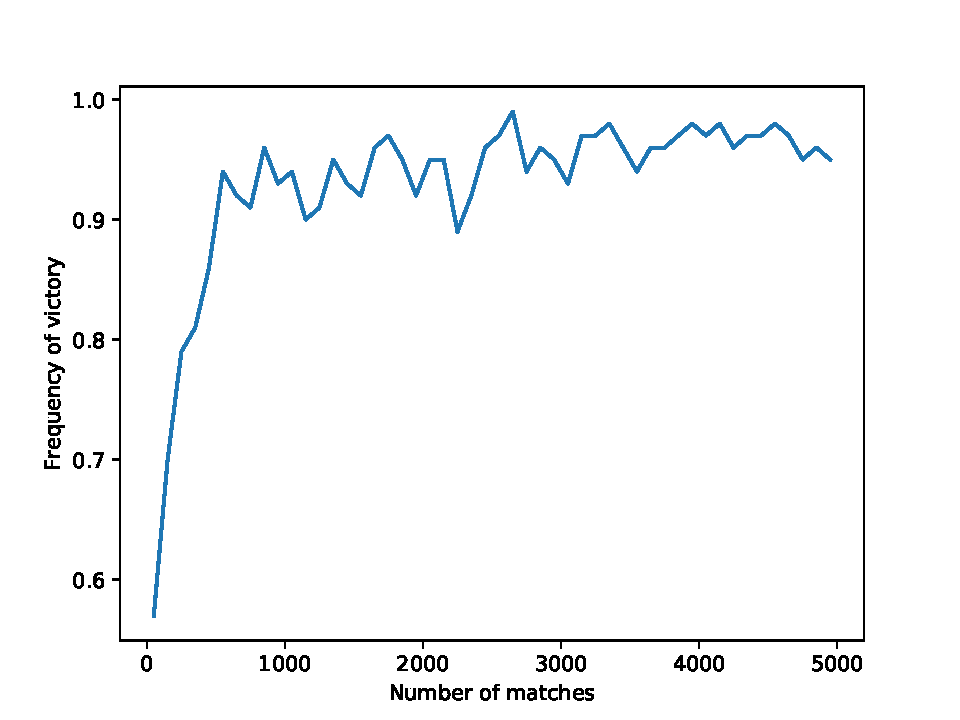
\includegraphics[width=0.95\columnwidth]{images/learning_curve_against_random.pdf}
    \caption{\label{learning_curve_against_random}The learning curve of the RL agent against a random one.}
\end{figure}

To analyze the learning time of the \emph{RL} agent, we simulate it against the \emph{Random} agent.
At the beginning, the \emph{RL} agent knows nothing.
We run $5000$ games, and we compute the frequency of victories for the \emph{RL} agent for every chunk of $100$ games.
The results are presented on Figure~\ref{learning_curve_against_random}.
As we can see, with only a few hundreds games, this agent is far better than the \emph{Random} one.

\subsubsection{Performance of the agents}

We simulated $1000$ games between each pair of agents.
The results are presented in Table~\ref{comparative_table}.
When the sum of the scores isn't equal to $1000$, it means that games ended because both agents died at the same time.

As can be seen, the \emph{Minimax} agent is nearly unbeatable, no agent scored a point against it.
However, it scored $933$ against the \emph{Random} agent, which means that it was killed $77$ (while killing the other one).
Even though the \emph{RL} dies $4$ times out of $1000$ without killing the \emph{Random} agent, it performs better with respect to its own score.
In $991$ out of $1000$ games, it manages to stay alive while killing its opponent, which means it learned from experience to avoid going too close to its opponent, whereas the $emph{Minimax}$ agent thinks its opponent will take the best action.
This hypothesis is clearly false for the \emph{Random} agent.

\begin{table}[h]
	\caption{\label{comparative_table}Results of the games.}
	\centering
	\begin{tabular}{llll}
		\hline
        \textbf{Game} & \textbf{Random} & \textbf{Minimax}  \\
		\hline
        \textbf{RL} & 991 - 4 & 0 - 174 \\
        \textbf{Minimax} & 933 - 0 &  \\
		\hline
	\end{tabular}
\end{table}

\begin{figure}[h]
	\centering
    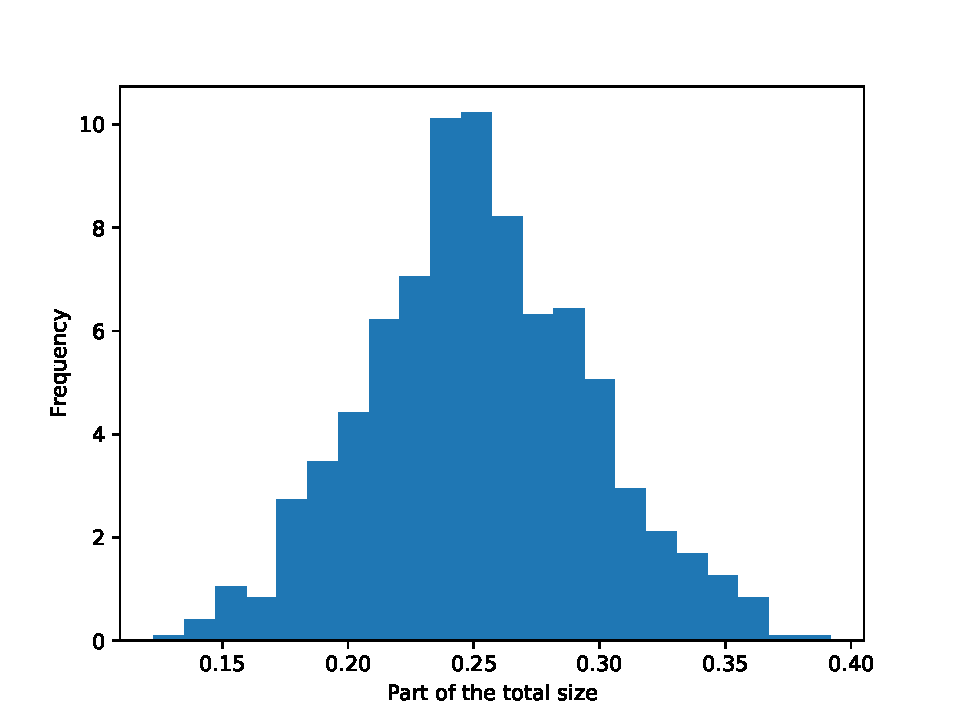
\includegraphics[width=0.95\columnwidth]{images/histo_size.pdf}
    \caption{\label{histo_size}Distribution of the proportion of the size of the \emph{RL} agent for the $776$ games ended after $1000$ iterations.}
\end{figure}

The game between the \emph{RL} and \emph{Minimax} agents ends before $1000$ iterations $174$ times out of $1000$.
For $50$ of theses games, it ends in a tie, where both agents are killed at the same iteration.
The other $776$ games are interesting to look at.
When a game reaches the maximum number of iterations, we stop it, and measure the sizes of the two agents.
The distribution of the proportion of the size of the \emph{RL} agent compared to the sum of both sizes is presented on Figure~\ref{histo_size}.
The main difference between the \emph{RL} agent and the \emph{Minimax} one is the local vision of the former, which can only ``see'' candies and snakes up to a Manhattan distance of $8$ and $4$ squares.
The average propotion size of $25$ \% for the \emph{RL} agent is thus really strong.

\subsection{Performance of our Agent in the ALife Environment}

We only tried to deploy our \emph{RL} agent in the ALife Environment since it is model-free.
Deploying the \emph{Minimax} agent would have require to create a totally new model, which would have made it a different agent.
When using the same technics (Q-Learning or SARSA, $\epsilon$-greedy or Softmax exploration), the results aren't as satisfactory as in the Snake world.
This environment is much more complicated, and the inputs and outputs are analogous.

We chose to tackle these issues by discretizing the inputs.
We don't use the energy input.
We multiply each other input (the color sensors) by $5$, and round them to the lower integer.
To keep the number of actions small, we only allow rotations of $-\frac{\pi}{2}$, $0$, $\frac{\pi}{2}$ and $pi$.

After a few minutes of simulation, it seems that the herbivore have understood that they have to eat the plants.
Unfortunately, this timeframe doesn't seem sufficient enough for the insects to learn other lessons.

\section{Conclusion and Future Work}
    This environment is interesting to use for multiple agents, because it has a few aspects.
    A snake has to eat candies to grow, but in the same time it also has to avoid collisions with walls and other snakes.
    The inputs defined in Subsection~\cite{rl_agent} allows an agent to have a local but precise vision of its environment.
    Such an agent learns quickly and is able to outperform a \emph{Random} agent after a few hundreds games.
    When competing against a strong AI, the \emph{Minimax} agent, whose only limitation is the depth it can explore when deciding which action to take, its results are quite satisfactory.

    The main issue with the strategy we chose is the high number of states.
    For instance, the agent has to learn many times that going into a wall is bad, because there are a lot of different states where it is touching a wall.
    To continue this work, one should focus on Deep Reinforcement Learning, to give the snake a bigger vision of its environment, and make it easier and quicker for it to learn the best strategy.

\begin{thebibliography}{4}

	\bibitem{lecture-rl} % Web document
	N.~Tziortziotis. Lecture IV - Introduction to Reinforcement Learning. \textit{INF581 Advanced Topics in Artificial Intelligence}, 2018.

	\bibitem{lecture-rl2} % Web document
	N.~Tziortziotis. Lecture V, part II - Approximate and Bayesian Reinforcement Learning. \textit{INF581 Advanced Topics in Artificial Intelligence}, 2018.

	\bibitem{qlearning}
	Watkins, Christopher \& Dayan, Peter. (1992). Technical Note: Q-Learning. Machine Learning. 8. 279-292. 10.1007/BF00992698. 

	\bibitem{sarsa}
	A. Rummery, G \& Niranjan, Mahesan. (1994). On-Line Q-Learning Using Connectionist Systems. Technical Report CUED/F-INFENG/TR 166. 

    \bibitem{intro-rl}
    Sutton, R. S. \& Barto, A. G. 1998 Reinforcement learning: an introduction. Cambridge, MA: MIT Press.
	
	\bibitem{lecture_minimax}
	N.~Tziortziotis. Lecture III - Structured Output Prediction \& Search and Optimization. \textit{INF581 Advanced Topics in Artificial Intelligence}, 2018.
\end{thebibliography}

\end{document}
